\section{Information Theory}

\begin{defn}
    \newterm{Information} is $I = -\log p(x)$
\end{defn}

\begin{defn}
    \newterm{Entropy} is the functional $H[p] = - \sum p(x) \log p(x) = E_p[log p(x)]$.
\end{defn}

\begin{defn}
    \newterm{Differential Entropy} is the functional $H[p] = - \int p(x) \log p(x) \dx$
\end{defn}

\begin{defn}
    \newterm{KL Divergence} (also known as \newterm{relative entropy} between a distribution $p$ and $q$ is
    
    \begin{align}
        \kldiv{p}{q} &= -\int p(x) \log q(x) + \int p(x) \log p(x) \dx  \\
        &= H[p, q] - H[p]
    \end{align}
\end{defn}

We can further simplify this as

\begin{align}
    \kldiv{p}{q} &= -\int p(x) \log q(x) + \int p(x) \log p(x) \dx  \\
    &= \int p(x) (\log p(x) - \log q(x)) \dx \\
    &= \int p(x) \log \frac{p(x)}{q(x)} \dx \\
    &= - \int p(x) \log \frac{q(x)}{p(x)} \dx.
\end{align}

Note that last two equations differ only in the minus sign, which flips the fraction.

\begin{thm}
The KL-divergence is invariant under parameter transformations \todo{proof}.
% https://en.wikipedia.org/wiki/Kullback%E2%80%93Leibler_divergence
\end{thm}

\begin{tcolorbox}
    Looking at the definition of entropy for each, we can view $\kldiv{p}{q}$ as sort of $H[q] - H[p]$, which would be
    
    \begin{align}
        H[q] - H[p] &= -\int q(x) \log q(x) \dx - \left( -\int p(x) \log p(x) \dx \right)
    \end{align}
    
    But since KL-divergence can be thought of as relative distance with respect to $p$, this turns into
    
    \begin{align}
        -\int p(x) \log q(x) \dx - \left( -\int p(x) \log p(x) \dx \right) = H[p, q] - H[p].
    \end{align}
\end{tcolorbox}

\subsection{Properties of the KL-divergence}

\begin{thm}
The KL-divergence is always positive.
\end{thm}

\begin{proof}
    % https://stats.stackexchange.com/questions/335197/why-kl-divergence-is-non-negative
    \begin{align}
        0 \leq \kldiv{p}{q} = - \int p(x) \log \frac{q(x)}{p(x)} \dx
    \end{align}
\end{proof}

\begin{thm}
$\kldiv{p}{q} \neq \kldiv{q}{p}$
\end{thm}


\begin{tcolorbox}
Explain KL-divergence as a relative distance. 

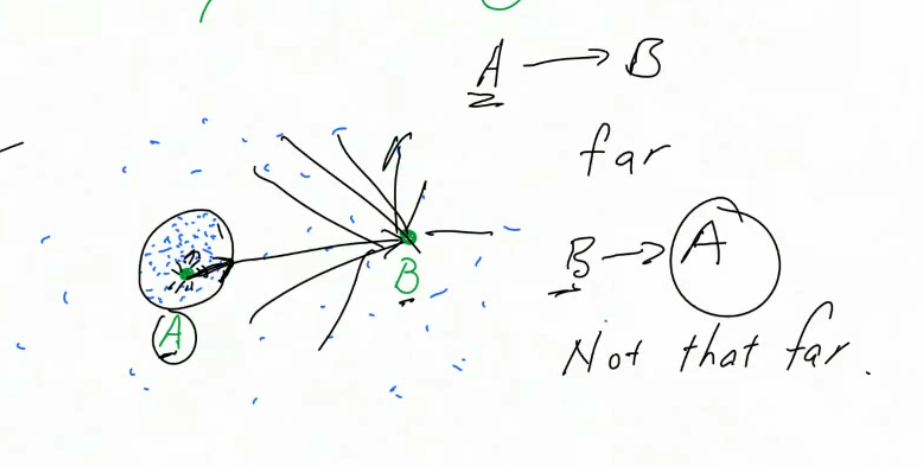
\includegraphics[width=0.7\textwidth]{img/kldivergence-relative}
\end{tcolorbox}



\subsection{Relationship between $\log p(x)$ and $D_{KL}$}

Let's say we have a distribution $p(z | x)$ which we don't know, and we want to use $q(z)$ to estimate it. We use the KL-divergence to measure the quality of the esimate, that is $\kldiv{q(z)}{p(z|x)}$.

\begin{align}
    \label{eq:kldiv}
    \kldiv{q(z)}{p(z|x)} = - \int q(z) \log \frac{p(z|x)}{q(z)} \dz
\end{align}

We know from conditional probability that

\begin{equation}
    \frac{p(x,z)}{p(x)} = p(x|z)
\end{equation}

and plugging that back into \ref{eq:kldiv} we get

\begin{align}
    \kldiv{q(z)}{p(z|x)} &= - \int q(z) \log \frac{p(z|x)}{q(z)} \dz \\
    &= - \int q(z) \log \left( \frac{p(x,z)}{p(x)}  \frac{1}{q(z)} \right) \dz \\
    &= - \int q(z) \left( \log \frac{p(x,z)}{q(z)} + \log \frac{1}{p(x)} \right) \dz \\
    &= - \int q(z) \log \frac{p(x,z)}{q(z)} \dz - \int q(z) \log \frac{1}{p(x)} \dz \\
    &= - \int q(z) \log \frac{p(x,z)}{q(z)} \dz + \int q(z) \log p(x) \dz \\
    &= - \int q(z) \log \frac{p(x,z)}{q(z)} \dz + \log p(x) \int q(z) \dz \\
    &= - \int q(z) \log \frac{p(x,z)}{q(z)} \dz + \log p(x)
\end{align}

and moving the first term to the left side of the equation gives us

\begin{equation}
    \kldiv{q(z)}{p(z|x)} + \int q(z) \log \frac{p(x,z)}{q(z)} \dz = \log p(x).
\end{equation}

We call the second quantity on the left the \newterm{variational lower bound} (also known as ELBO for \newterm{expected lower bound}) and we denote it as $\gL$. For clarity, let us denote $D_{KL} = \kldiv{q(z)}{p(z|x)}$ in the rest of this section.

\begin{equation}
    D_{KL} + \gL = \log p(x).
\end{equation}

Here we make a few observations. First of all, note that $\gL = -D_{KL}$ \todo{je tohle fakt pravda?}, which is always negative. The initial KL-divergence is always positive, and since $0 < p(x) < 1$ \todo{tohle ale neni nutne pravda pro density? pro diskretni to ale plati ... tzn domyslet continuous case} we get $\log ([0; 1])$ on the right, which is always negative.

\begin{equation}
    \underbrace{D_{KL}}_{\text{always +}} + \underbrace{\gL}_{\text{always -}} = \underbrace{\log p(x)}_{\text{always -}}
\end{equation}

Because we started with $p(z|x)$ we know $x$ is some fixed value which does not change as we optimize $q(z)$ to approximate it. This means the right side $\log p(x)$ is also fixed. As a result, changing $\gL$ will change the value of $D_{KL}$ which matches our intuition.

A key insight here is that increasing $\gL$ immediately decreases $D_{KL}$, because $\gL$ is negative, $D_{KL}$ is positive, and $\log p(x)$ does not change as $q(z)$ changes. As a result, directly optimizing $\gL$ allows us to indirectly lower $D_{KL}$ and improve our estimate $q(z)$ of $p(z|x)$.

\subsection{Useful inequalities}

\begin{thm}[Log-sum inequality]
TODO
% https://en.wikipedia.org/wiki/Log_sum_inequality
\end{thm}

\begin{thm}[Gibbs' inequality]
TODO
% https://en.wikipedia.org/wiki/Gibbs%27_inequality
\end{thm}

\begin{thm}[Jensen inequality]
% https://en.wikipedia.org/wiki/Jensen's_inequality
\end{thm}



\section{Expectation-Maximization (EM) algorithm}

MLE (or MAP) when some data is missing (hidden).

\begin{itemize}
    \item Given: $X = (x_1, \dots, x_n)$
    \item Model: $(X, Z) \sim p_\theta$ for some (unknown) $\theta \in \Theta$. \item Typically $p_\theta$ is from the exponential family.
    \item Goal: $\theta_{\text{MLE}} = argmax_\theta p_\theta(x)$
    \item Issue: $p_\theta = \int_\theta p_\theta(x,z)$ is difficult to maximize. This could mean $p_\theta$ is multi-modal for example, and differentiating leads to an implicit equation which is impossible to solve analytically.
    \item Alg: initialize $\theta_0 \in \Theta$, for $t = 0,1,2,\dots$ do:
        \begin{itemize}
            \item E-step: $Q(\theta, \theta_t) = E_{\theta_t} [\log p_\theta(X, Z) | X = x]$.
            \item M-step: $\theta_{t+1} = argmax_\theta Q(\theta, \theta_t)$.
        \end{itemize}
        
    \item Pros:
        \begin{itemize}
            \item $p_{\theta_{t+1}}(x) \geq p_{\theta_t}(x)$.
            \item Works well in practice.
        \end{itemize}
    
    \item Cons:
        \begin{itemize}
            \item Not guaranteed to give $\theta_{\text{MLE}}$, because it might get stuck in local optima.
            \item MLE might overfit, but it is possible to do MAP.
            \item Convergence can be slow.
            \item Specialized to exponential families
        \end{itemize}
\end{itemize}

Now the derivation:

\begin{itemize}
    \item Goal: $\arg \max_\theta p_\theta(x)$
    \item Specialize: $p_\theta(x, z) = e^{g(\theta)^T s(x,z)} h(x, z) / c(\theta)$.
    \item Note that the MLE is invariant under reparameterization \todo{proof}. As such, it is sufficient to consider $\theta = g(\theta)$.
    \item Natural form: $p_\theta(x, z) = e^{\theta^T s(x,z)} h(x,z) / c(\theta)$.
\end{itemize}

\begin{equation}
    0 = \frac{\partial}{\partial \theta_i} \log p_\theta(x) = \frac{1}{p_\theta(x)} \sum_z \frac{\partial}{\partial \theta_i} p_\theta(x, z)
\end{equation}

\begin{align}
    \frac{\partial}{\partial \theta_i} p_\theta(x, z) &= \frac{\partial}{\partial \theta_i} e^{\theta^T s - \log c(\theta)} \underbrace{h(x,z)}_{\text{constant}} \\
    &= \left(s_i(x,z) - \frac{\partial}{\partial \theta_i} \log c(\theta) \right) e^{\theta^T s(x,z)} h(x,z) \\
    &= \left(s_i(x,z) - \frac{\partial}{\partial \theta_i} \log c(\theta) \right) p_\theta(x, z)
\end{align}

Now using the property of the exponential family \todo{proof} we get the expected value of the i-th sufficient statistic.

\begin{equation}
    \frac{\partial}{\partial \theta_i} \log c(\theta) = E_\theta[s_i(X, Z)]
\end{equation}

Now continuing our previous derivation

\begin{align}
    0 &= \frac{1}{p_\theta(x)} \sum_z \frac{\partial}{\partial \theta_i} p_\theta(x, z) \\
    &= \frac{1}{p_\theta(x)} \sum_z \left( s_i(x,z) - E_\theta[s_i(X, Z)] \right) p_\theta(x, z) \\
    &= \sum_z s_i(x, z) p_\theta(z | x) - \sum_z  E_\theta[s_i(X, Z)] p(z | x) \\
    &= \sum_z s_i(x, z) p_\theta(z | x) - E_\theta[s_i(X, Z)] \\
    &= E_\theta[s_i(X, Z) | X=x] - E_\theta[s_i(X, Z)].
\end{align}

As a result, we get an implicit equation

\begin{equation}
    E_\theta[s_i(X, Z) | X=x] = E_\theta[s_i(X, Z)].
\end{equation}

The above equation can't be solved analytically. This leads us to an iterative approach \todo{why?}.

Algorithm:

\begin{itemize}
    \item Let $\theta_0 \in \Theta$
    \item For $t = 1, 2, 3, \dots$
    \item Solve $E_{\theta_{t-1}}[s_i(X,Z) | X=x) = E_{\theta_t}[s_i(X,Z)$ for $\theta_t$.
\end{itemize}

---

\begin{itemize}
    \item $Q(\theta, \theta_0) = E_{\theta_0} [ \log p_\theta(X,Z) | X = x]$
    \item $p_\theta(x, z) = e^{\theta^T s(x,z) - \log c(\theta)} h(x,z)$
    \item $\log p_\theta(x, z) = \theta^T s(x,z) - \log c(\theta) + \log h(x,z)$
    \item $E[\log p_\theta(X,Z) | X=x] = \theta^T E_{\theta_0}[s(X, Z) | X=x] - \log c(\theta) + const$
    \item $0 = \frac{\partial}{\partial \theta_i} E_{\theta_0}[s_i(X, Z) | X=x] - E_\theta[s_i(X,Z)$
    \item and we get exactly as what we had before.
\end{itemize}


\section{Estimators}

Assume $D = (X_1, X_2, \dots, X_n)$.

\begin{defn}
    A \newterm{statistic} is a random variable $\rS$ that is a function of the data $D$ (i.e. $S = f(D)$).
\end{defn}

\begin{defn}
    An \newterm{estimator} is a statistic intended to approximate a parameter generating the distribution of the data $D$.
\end{defn}

Notation:

\begin{itemize}
    \item $\hat{\theta}$ denotes an estimator of $\theta$.
    \item $\hat{\theta_n}$ emphasizes the dependence of the estimator on $n$.
\end{itemize}

\begin{defn}
    The \newterm{bias} of an estimator $\hat{\theta}$ is
    
    \begin{equation}
        bias(\hat{\theta}) = E \hat{\theta} - \theta.
    \end{equation}
\end{defn}

\begin{defn}
    An estimator is \newterm{unbiased} if $bias(\hat{\theta}) = 0$.
    
    \todo{zkusit ukazat u sample mean unbiased a sample variance biased}
\end{defn}

\subsection{Decision theory terminology}

\begin{itemize}
    \item Decision rule $\delta$
        \begin{itemize}
            \item State is unknown $s$.
            \item Data $D$ is observed (or $X$).
            \item Action $a = \delta(D)$ is chosen using the data $D$.
            \item Loss $L(s, a)$ is incured as a result of choosing the action.
        \end{itemize}
    \item Estimators - Estimator fn $g$
        \begin{itemize}
            \item Parameters $\theta$
            \item Data $D$
            \item Estimator/Estimate $\hat{\theta} = g(D)$. Estimator is a random variable (in which case $\hat{\theta}$ is also random variable. Estimate is a value of the estimator for particular data.
            \item Loss $L(\theta, \hat{\theta})$.
        \end{itemize}
            \begin{itemize}
                \item Target value $Y$
                \item Observe point $X$
                \item Prediction $\hat{Y} = f(X)$
                \item Loss $L(Y, \hat{Y})$
            \end{itemize}
    \item Regression/Classification - Prediction fn $f$
\end{itemize}

TODO: unity notation between random variable and a specific value (sample) of the variable.


\subsection{Loss and Risk}

$D = (X_1, \dots, X_n), D \sim p_\theta, \theta \sim \pi, \hat{\theta} = f(D) = \delta(D)$.

$Loss = L(\theta, f(D))$, but since $\theta$ and $D$ are random variables, this is not well defined. We can either:

\begin{itemize}
    \item \newterm{Bayesian expected loss} is $p(\pi, f(D)) = E[L(\theta, f(D)) | D]$, averaging over $\theta$.
    \item \newterm{Frequentist risk} is $R(\theta, f) = E[L(\theta, f(D)) | \theta]$, averaging over $D$.
\end{itemize}

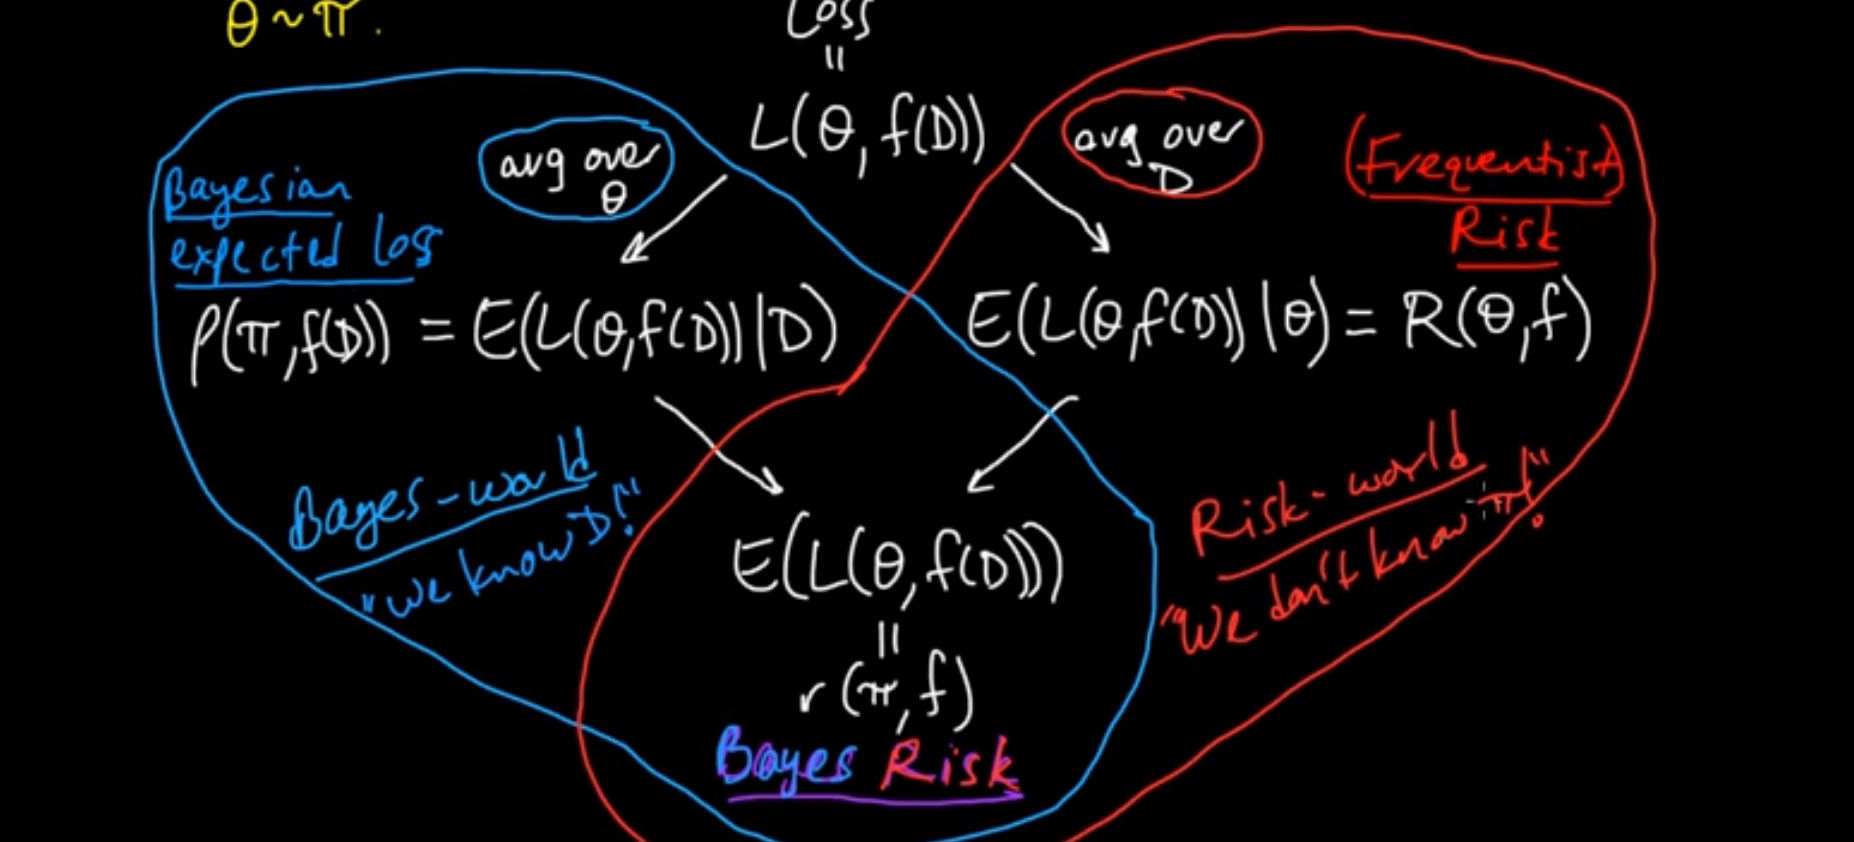
\includegraphics[width=0.7\textwidth]{img/loss-and-risk}

\begin{itemize}
    \item Bayesian: Assume prior $\pi$
        \begin{itemize}
            \item Case 1: Know $D$. Choose $f(D)$ to minimize $p(\pi, f(D))$.
            \item Case 2: (Conditional Bayes). Don't know $D$. Choose $f$ to minimize $r(\pi, f)$.
        \end{itemize}
        
    \item Frequentist: Introduce a further principle to guide the choice.
        \begin{enumerate}
            \item Unbiasedness
            \item Admissibility
            \item Minimax (minimizing the maximum possible risk)
            \item Invariance
        \end{enumerate}
\end{itemize}


\subsection{Bias-Variance Decomposition}

$MSE = bias^2 + var$

\begin{defn}
    The \newterm{mean-squared error} (\newterm{MSE}) of an estimator $\hat\theta = f(D)$ for $\theta$ is $MSE(\hat\theta) = E[(\hat\theta - \theta)^2 | \theta]$. This is just risk $r(\theta, f)$ under square loss.
\end{defn}

Recall: $bias(\hat\theta) = E \hat\theta - \theta$.

\begin{thm}
    $MSE(\hat\theta) = bias(\hat\theta)^2 + var(\hat\theta)$.
\end{thm}

\begin{proof}
    Let $\mu = E\hat\theta$, then

    \begin{align}
        E[(\hat\theta - \theta)^2] &= E[(\hat\theta - \mu + \mu - \theta)^2] \\
        &= E[((\hat\theta - \mu) + (\mu - \theta))^2] \\
        &= E[(\hat\theta - \mu)^2 + 2 (\hat\theta - \mu)(\mu - \theta) + (\mu - \theta)^2] \quad \text{making use of $\mu = E\hat\theta$}\\
        &= E(\hat\theta - \mu)^2 + (\mu - \theta)^2 \\
        &= var(\hat\theta) + bias(\hat\theta)^2
    \end{align}
\end{proof}

\begin{defn}
    Given decision rules $\delta, \delta'$ we say $\delta$ \newterm{dominates} $\delta'$ if $R(\theta, \delta) \leq R(\theta, \delta') \forall \theta$, and $R(\theta, \delta) < R(\theta, \delta')$ for some $\theta$.
\end{defn}

\begin{defn}
    A decision rule $\delta$ is \newterm{inadmissable} if there is another decision rule that dominates $\delta$. Otherwise, $\delta$ is \newterm{admissable}.
\end{defn}

\subsection{Bayesian Decision Theory}

\begin{align*}
    p(\pi, \delta(D)) &= E[L(\theta, \delta(D)) | D] \\
    r(\pi, \delta) &= E[L(\theta, \delta(D))] \\
    &= E[E[L(\theta, \delta(D)] | D] \\
    &= E[p(\pi, \delta(D))]
\end{align*}

\begin{tcolorbox}
    Informally: (\url{https://en.wikipedia.org/wiki/Bayes_estimator#Generalized_Bayes_estimators})
    
    \begin{itemize}
        \item A \newterm{generalized Bayes rule} is a decision rule $\delta$ minimizing $p(\theta, \delta(D))$ for each $D$.
        \item A \newterm{Bayes rule} minimizes $r(\theta, \delta)$.
        \item $GBR \implies BR$, but $BR \nRightarrow GBR$.
        \item If $r(\pi, \delta) = \inf \forall \delta$, then anything is a BR, but a GBR still makes sense.
        \item On sets of $\pi$-measure $0$, then BR is arbitrary, but GBR is still sensible.
    \end{itemize}
\end{tcolorbox}

Complete class theorems: Under mild conditions, every GBR (for a proper $\pi$) is admissible. Furthermore, ever admissible decision rule is a GBR for some prior $\pi$ (possibly improper).